\documentclass[Thesis,Final,NoHardback]{mpThesis}

\usepackage{longtable}
\usepackage{booktabs}
\usepackage{graphicx}
\usepackage{siunitx}
\usepackage{graphicx}
\usepackage{float}
\usepackage{tabularx}
\usepackage{array}
\usepackage[final]{microtype}
\setlength{\emergencystretch}{3em}
\let\cleardoublepage\clearpage
\geometry{left=22mm,right=22mm,top=24mm,bottom=24mm,heightrounded}
\hypersetup{colorlinks=true,urlcolor=blue,linkcolor=black,citecolor=black}
\captionsetup[table]{justification=raggedright,singlelinecheck=false}
\captionsetup[figure]{justification=raggedright,singlelinecheck=false}
% keep table/figure numbers continuous so the in-text references (Table 1 ... Table 12)
% match the captions exactly
\counterwithout{table}{chapter}
\counterwithout{figure}{chapter}
\renewcommand{\thetable}{\arabic{table}}
\renewcommand{\thefigure}{\arabic{figure}}
\renewcommand{\labelitemi}{\textbullet}

\StudentName{ZHANG XIANG}
\StudentNumber{P2600300}
\AcademicUnit{Faculty of Applied Sciences}
\Programme[Doctor of Philosophy in Artificial Intelligence Driven Drug Discovery]{Doctor of Philosophy in Artificial Intelligence Driven Drug Discovery}
\Supervisor{\textemdash}
\Cosupervisor{\textemdash}

\Title[MOCHI: A Self-Evolving Multi-Agent System for End-to-End AI Drug Discovery]{MOCHI: A Self-Evolving Multi-Agent System for End-to-End AI Drug Discovery}
\ThesisNumber{0000}{AIDD}{FCA}{zhang}{mochi}
\ThesisKeywords{multi-agent systems, AI drug discovery, retrosynthesis, enzyme engineering, laboratory automation}
\Date{2026-11-16}

\begin{document}
\nocite{r01,r02,r03,r04,r05,r06,r07,r08,r09,r10,r11,r12,r13,r14,r15,r16,r17,r18,r19,r20,r21,r22}

\begin{FrontMatter}[FigLs=false,TabLs=false,AbbreLs=false]
\chapter{Abstract}

Artificial-intelligence drug discovery (AIDD) now generates more candidate targets, molecules and protocols than any single researcher can triage, yet the tools that produce them are disjoint and the reasoning that connects them is rarely auditable. We present MOCHI (Multi-agent Orchestrator for Chemical and biomedical Intelligence), a self-evolving multi-agent system in which a manager, a developer, a critic and a tool-creation agent collaborate over a shared ocean of 46 scientific tools. MOCHI is deliberately scenario-agnostic: four interchangeable stage programs cover (i) downstream effector-target discovery, (ii) structure-guided enzyme variant design, (iii) multi-step retrosynthesis planning and (iv) compilation of wet-lab protocols into validated self-driving-laboratory (SDL) instructions. A deterministic critic audit, a provenance record of every database call and a dual offline/online engine make every run reproducible and inspectable.

On four real tasks MOCHI recovers a Wnt/Notch receptor-class shortlist that motivated the experimental validation of the Wnt co-receptor LRP6, ranks the experimentally validated best strictosidine-synthase variant first out of 2,773 candidates, plans a two-step synthesis of lidocaine and a three-step synthesis of benorilate (all eight benchmark drugs solved), and compiles six clean protocols while catching five of five deliberately corrupted ones. Ablations show that dynamic tool creation is required for the target task and that the experimental prior is required to place the true best variant first. The run artefacts and the command that rebuilds every table and figure are available at \url{https://github.com/simmzx/mochi}, and a single command reproduces the whole suite.

\Keywords{multi-agent systems, AI drug discovery, retrosynthesis, enzyme engineering, laboratory automation, reproducibility}

\end{FrontMatter}

\begin{MainMatter}
\chapter{Introduction}\label{ch:1}

\section{The data-to-decision bottleneck in AIDD}

Drug discovery has been transformed by data: a modern programme can query a protein's structure, its expression across thousands of tumours, its interaction partners, its chemical ligands and its literature within minutes. What has not scaled is the translation of those data into a defensible decision. A target is worth pursuing only if it is linked to the disease, mechanically plausible, druggable and still novel; a mutation is worth synthesising only if it is close enough to the active site to matter yet conservative enough to fold; a route is worth running only if every leaf is purchasable; a protocol is worth automating only if every volume and temperature is physically feasible. Each of these judgements requires the same three ingredients - heterogeneous evidence, explicit domain constraints and a written rationale - and each is currently assembled by hand.

Large language models (LLMs) are attractive precisely here, because they can plan, call tools and write the rationale \cite{r01,r02}. Yet a single model with a bag of tools is a poor fit for regulated scientific reasoning: it may hallucinate a number, silently skip a control, or change its answer between runs. The engineering question of this project is therefore not 'can an LLM call a database?' but 'can a multi-agent system make scientific decisions that are reproducible, auditable and correctable?'

\section{Agentic systems for biomedical research}

Tool-augmented LLMs were formalised by ReAct, which interleaves reasoning traces with actions \cite{r01}, and by Toolformer, which learns when to call APIs \cite{r02}. Chemistry-specific systems followed: ChemCrow combines 18 expert tools under an LLM planner \cite{r03}, and Coscientist closed the loop from literature to robotic execution \cite{r04}. In biology, BioDiscoveryAgent designs genetic perturbation experiments \cite{r05}, and self-evolving frameworks that maintain a growing tool library have recently been proposed for biomedical research \cite{r06,r07}. These systems share a design pattern - a planner, a set of tools, an evaluator - but differ in how much autonomy the model is given.

Three weaknesses recur across this literature. First, evaluation is usually a single task: a system tuned for chemistry is not shown to plan a CRISPR screen. Second, the evaluator is itself an LLM, so a confident but wrong plan can pass review. Third, reproducibility is rarely demonstrated: the tool outputs behind a claim are usually not preserved. The present work addresses all three by treating the orchestration layer as a first-class engineering artefact: explicit stage contracts, a deterministic audit with veto power, and a provenance log for every external call.

\section{Why four scenarios}

We deliberately chose four tasks that stress different parts of the same orchestration problem (Table 1). Target discovery is evidence integration under uncertainty; enzyme design is structure-constrained combinatorial search with experimental feedback; retrosynthesis is graph search with hard feasibility constraints; protocol compilation is translation from natural language into a typed, checkable program. If one orchestrator handles all four, it is a platform rather than a demo.

\begin{table}[htbp]
\centering
\small
\caption{The four scenarios share one orchestrator and differ only in their stage programs and tools.}
\begin{tabularx}{\textwidth}{l>{\raggedright\arraybackslash}X>{\raggedright\arraybackslash}X>{\raggedright\arraybackslash}X>{\raggedright\arraybackslash}X}
\hline
Scenario & Input & Core computation & Output & Failure mode exercised \\
\hline
S1 Target discovery & anchor gene + disease & 6-dimension evidence scoring over public omics & ranked effectors + dossier & missing capability (no competence scorer) \\
S2 Enzyme design & enzyme + round-1 data & structure/prior-guided variant scoring & 15-variant library + primers & experimental knowledge that a model lacks \\
S3 Retrosynthesis & target SMILES & template-based best-first AND-OR search & shortest route to stock & combinatorial explosion / dead ends \\
S4 Protocol $\rightarrow$ SDL & natural-language protocol & typed compilation + static validation & validated SDL program & silent unit/safety errors \\
\hline
\end{tabularx}

\end{table}

\section{Contributions}

\begin{itemize}
\setlength{\itemsep}{0pt}\setlength{\parskip}{0pt}
\item A scenario-agnostic, self-evolving multi-agent architecture (manager, developer, critic, tool creator) in which the critic's audit is deterministic Python and has veto power over the language model.
\item A shared Tool Ocean of 46 tools spanning omics databases, structure analysis, cheminformatics and laboratory automation, with cached, provenance-logged access and a validation gate for generated tools.
\item Four independently runnable AIDD scenarios, each with a quantitative evaluation that includes a published ground truth (hindcast), a literature benchmark, or deliberately corrupted inputs.
\item A reproducibility contract: an offline deterministic engine, an OpenAI-compatible engine, and a single command that regenerates every number in this report from cached public data.
\end{itemize}


\chapter{Research Questions and Objectives}\label{ch:2}

The project is organised around three research questions that are answerable with the artefacts of a single run, rather than around a single predictive benchmark.

\begin{itemize}
\setlength{\itemsep}{0pt}\setlength{\parskip}{0pt}
\item RQ1 (generality). Can one orchestration layer drive four structurally different AIDD tasks - evidence integration, combinatorial design, graph search and program compilation - without task-specific agent code?
\item RQ2 (self-evolution). Does the ability to create a tool at runtime add capability that a static tool library cannot provide, and is the created tool trustworthy?
\item RQ3 (reliability). Does a deterministic critic audit combined with an explicit experimental prior improve the reliability of decisions compared with an unaudited, prior-free pipeline?
\end{itemize}

\section{Objectives and success criteria}

\begin{table}[htbp]
\centering
\small
\caption{Objectives are tied to a deliverable, a measurable success criterion and a results section.}
\begin{tabularx}{\textwidth}{l>{\raggedright\arraybackslash}X>{\raggedright\arraybackslash}X>{\raggedright\arraybackslash}X}
\hline
Objective & Deliverable & Success criterion & Where reported \\
\hline
O1  Build the orchestrator & 4 agents + stage registry + templates & one code path runs all four scenarios & §3, §4 \\
O2  Curate the tool ocean & 46 tools, cached, provenance-logged & every claim traceable to a call & §3.3, §7 \\
O3  Reproduce published science & hindcasts against two published results & recover the published answer or explain the miss & §4.1, §4.2 \\
O4  Validate feasibility outputs & route + SDL benchmarks & solved routes terminate in stock; corrupted protocols are caught & §4.3, §4.4 \\
O5  Demonstrate self-evolution & runtime tool creation & created tool passes 13/13 controls & §4.1, §4.5 \\
\hline
\end{tabularx}

\end{table}

The motivation for O3 deserves emphasis. A target-discovery system that is only judged on whether it produces 'a plausible list' is unfalsifiable. We therefore use published answers as a hindcast: the system is given exactly the information a researcher would have had before the answer was known, and we report whether, and at what rank, it recovers the known result.


\chapter{Methods and Materials}\label{ch:3}

\section{Architecture}

MOCHI separates the control plane from the data plane (Figure 1). The control plane decides what to do next; the data plane performs every computation that appears in the report. The manager is the only agent that sees the user's instruction; it retrieves a reasoning template by TF-IDF similarity, decomposes the task into four stages and delegates execution. The developer executes a stage program and may only change parameters from a whitelist. The critic runs a scenario-specific, deterministic audit and then asks the language model for a verdict; the stricter of the two wins, so the model cannot waive a failed control. When the audit reports a missing capability, the tool-creation agent researches, writes, tests and registers a new tool, and the affected stage is re-run.

\begin{figure}[htbp]
\centering
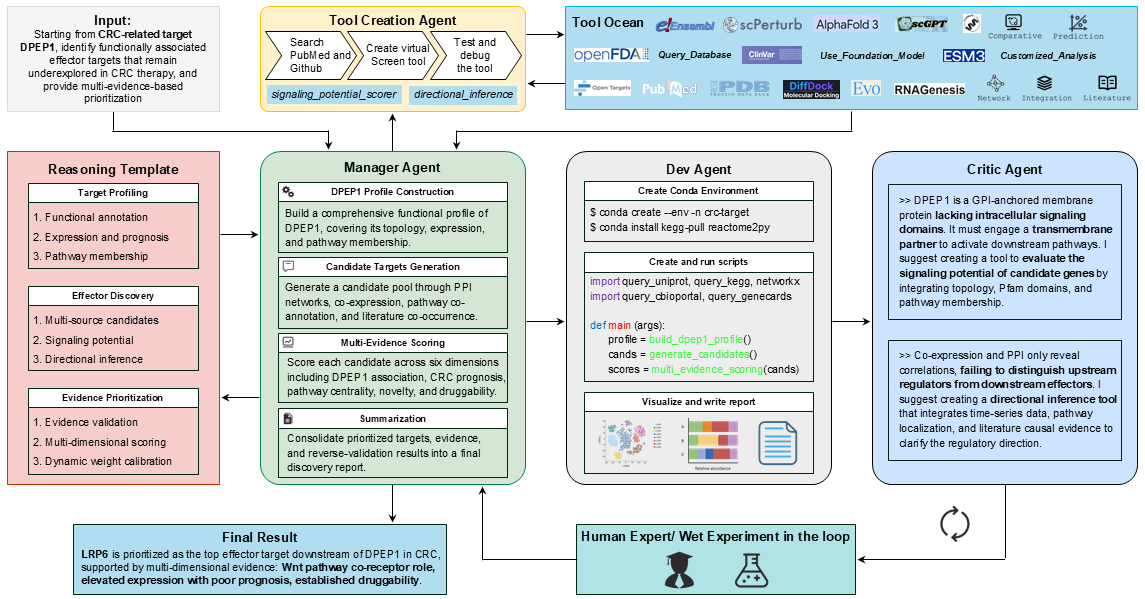
\includegraphics[width=0.99\textwidth]{figures/fig_workflow_ref.png}
\caption{The target-discovery workflow. The manager decomposes the DPEP1 task into profile construction, candidate generation, multi-evidence scoring and summarisation; the developer runs the stage programs and writes the artefacts; the critic audits each stage and asks for a new tool when a capability is missing; the tool-creation agent searches, builds and tests that tool before the stage is re-run. The final panel shows the hypothesis that the wet lab then tested; the quantitative evidence behind each step is reported in Section 4.}
\end{figure}

\section{Agents and their contracts}

Every agent call is a JSON contract, and the orchestrator parses only JSON. This is what allows the same agent classes to run against a real model, a local mock, or a rule-based engine: the contract, not the prose, carries the information.

\begin{table}[htbp]
\centering
\small
\caption{Agent contracts. The audit (Python) is evaluated separately from the verdict (model) and can override it.}
\begin{tabularx}{\textwidth}{l>{\raggedright\arraybackslash}X>{\raggedright\arraybackslash}X}
\hline
Call & Producer $\rightarrow$ consumer & Required fields \\
\hline
manager.plan & manager $\rightarrow$ orchestrator & stages\cite{r04} (name, goal, tools, criteria), hypotheses, reasoning \\
dev.plan & developer $\rightarrow$ stage program & steps, tools, parameter overrides (whitelisted) \\
critic.review & critic $\rightarrow$ manager & verdict (accept/revise/evolve), gaps, tool\_requests, weights \\
tool\_creation.design & tool creator $\rightarrow$ tool creator & tool name, algorithm, validation plan \\
manager.weights & manager $\rightarrow$ orchestrator & six weights summing to one \\
manager.synthesize & manager $\rightarrow$ report & narrative paragraph \\
\hline
\end{tabularx}

\end{table}

\section{Tool Ocean}

The Tool Ocean contains 46 deterministic tools in eleven categories (Table 4). Every tool returns a structured dictionary with an ok flag and a source string, never raises, and routes network access through one HTTP layer that caches responses for a week, retries with back-off, and appends the URL, parameters, status, latency and payload hash to provenance.jsonl. This single design decision is what makes the 'every number is traceable' claim in this report true.

\begin{table}[htbp]
\centering
\small
\caption{Tool Ocean by category. Counts exclude the runtime-created signalling-competence scorer.}
\begin{tabularx}{\textwidth}{l c >{\raggedright\arraybackslash}X}
\hline
Category & n & Representative tools \\
\hline
database & 12 & query\_uniprot, query\_opentargets\_associations, query\_cbioportal\_survival, query\_pubmed, query\_kegg\_pathways, resolve\_gene\_ids \\
chemistry & 6 & molecule\_properties, drugability\_score, query\_chembl\_target, query\_dgidb \\
literature & 5 & query\_pubmed\_cooccurrence, query\_pubmed\_novelty, citation\_network\_score \\
pathway / annotation & 8 & pathway\_coannotation, query\_quickgo, query\_interpro, pathway\_enrichment \\
network & 3 & query\_string, query\_intact, build\_ppi\_union \\
structure / sequence & 5 & fetch\_alphafold\_model, pocket\_geometry, conserve\_profile, primers, CDS mapping \\
retrosynthesis & 2 & one\_step\_disconnections, search\_route, route\_metrics \\
laboratory automation & 4 & parse\_protocol, compile\_sdl, validate\_sdl, simulate\_sdl \\
scoring & 1 & multi\_evidence\_scoring (plus the runtime-created competence scorer) \\
\hline
\end{tabularx}

\end{table}

\begin{figure}[htbp]
\centering
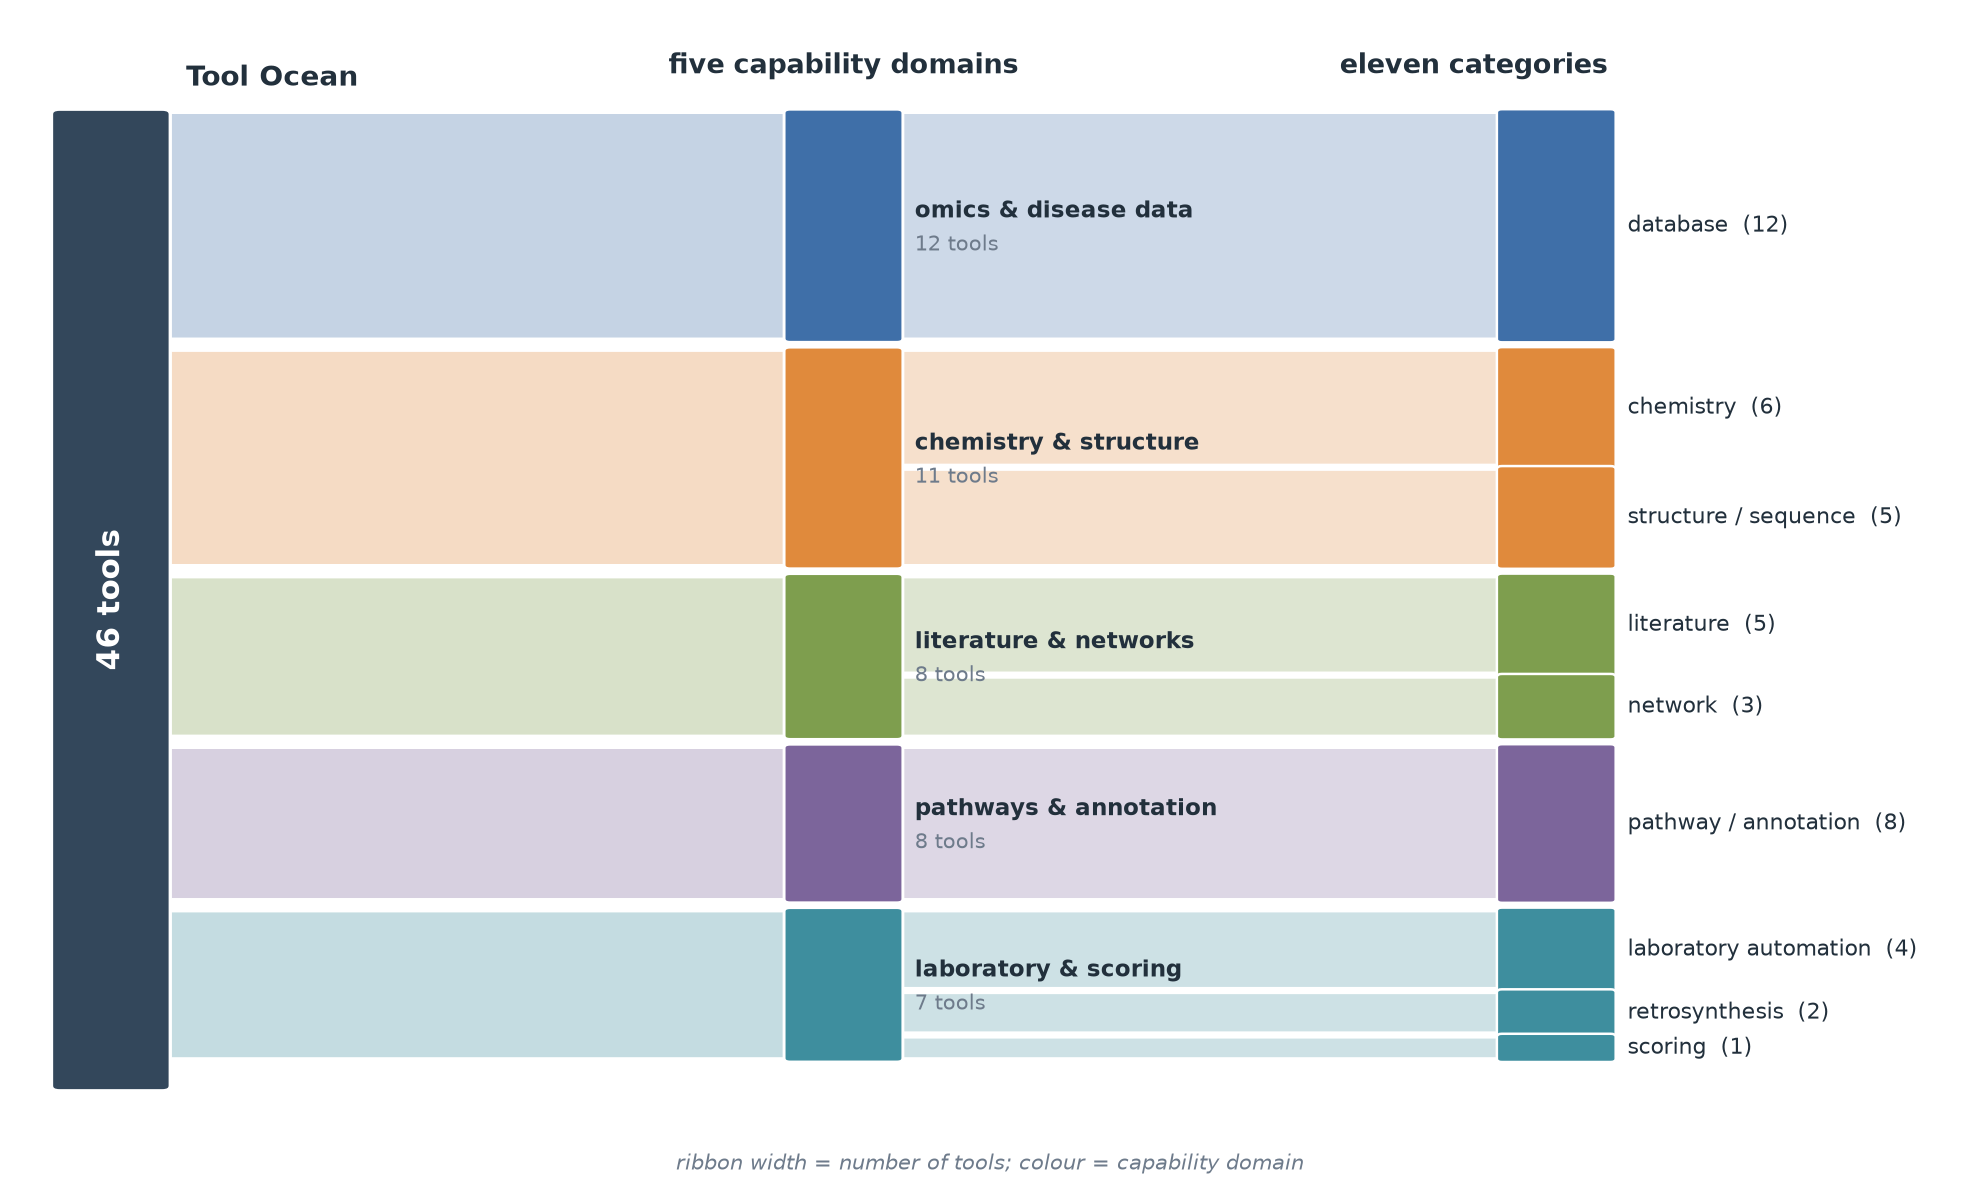
\includegraphics[width=0.99\textwidth]{figures/fig_sankey.png}
\caption{How the 46 tools of the Tool Ocean are distributed over five capability domains and the eleven categories. Ribbon width is proportional to the number of tools and the colour identifies the domain; the individual tools behind each category are listed in Table 4.}
\end{figure}

\section{Scenario adapters}

A scenario supplies four stage programs, an optional audit and an optional report renderer; nothing else changes. This is the entire mechanism by which MOCHI becomes a platform rather than a single-task agent. Table 5 summarises the stages.

\begin{table}[htbp]
\centering
\small
\caption{The four scenarios share the same four-stage skeleton.}
\begin{tabularx}{\textwidth}{l>{\raggedright\arraybackslash}X>{\raggedright\arraybackslash}X>{\raggedright\arraybackslash}X>{\raggedright\arraybackslash}X}
\hline
Stage & S1 target discovery & S2 enzyme design & S3 retrosynthesis & S4 protocol $\rightarrow$ SDL \\
\hline
Stage 1 & anchor profile: topology, expression, disease links & sequence, catalytic residues, AlphaFold model, homologs & target descriptors and functional-group inventory & sentence segmentation and typed step extraction \\
Stage 2 & candidate pool from PPI, co-expression, pathways, literature & all single substitutions within 12 A of the catalytic cluster & one-step disconnections from a curated template set & lowering to typed opcodes with SI units and devices \\
Stage 3 & signalling-competence scoring (created tool) & structure + chemistry + prior scoring & best-first AND-OR search to purchasable stock & static validation and bounded repair \\
Stage 4 & six-dimension ranking and evidence dossier & budgeted library, primers, hindcast & route ranking and literature benchmark & digital-twin simulation and corrupted-protocol benchmark \\
\hline
\end{tabularx}

\end{table}

\section{Decision models}

No stage delegates a computation to the language model. The models below are the actual decision rules; they were designed before the validation data were consulted and were not tuned on it.

Target discovery. Each candidate receives six dimension scores in [0,1] - association with the anchor, signalling competence, disease evidence, pathway centrality, novelty and druggability - and a weighted mean is taken over the dimensions that exist, multiplied by a coverage factor. Association combines physical interaction, expression co-variation, literature co-mention and specific pathway sharing with a noisy-OR, so that one strong channel is sufficient and absent channels do not dilute a real signal. Novelty is a saturating function of the number of PubMed records for the gene in the disease and overall, so a gene with no disease literature but 800 general papers is not counted as unexplored.

Enzyme design. A variant at position p with substitution wt$\rightarrow$mut receives score = leverage(d) $\times$ [0.55$\cdot$chemistry + 0.45$\cdot$prior] $\times$ (0.7 + 0.3$\cdot$packing) − 0.15$\cdot$conservation, where leverage = exp(−d/12) with d the minimum heavy-atom distance to the catalytic cluster, chemistry is a rescaled BLOSUM62 \cite{r15}, prior is the round-1 outcome for that position (hit 1.0 / reduced 0.5 / untested 0.5 / dead 0), packing penalises volume change and buried-glycine substitutions, and the conservation penalty comes from a Needleman-Wunsch alignment against 39 UniProt homologs.

Retrosynthesis. Six disconnection templates (amide, ester, aryl ether, N-alkylation, sulfonamide, nitro-to-amine interconversion) are applied by direct bond editing; the resulting fragments are sanitised, and a depth-limited best-first search terminates when every leaf is in a curated stock of commercially available building blocks \cite{r18,r20}.

Protocol compilation. A rule-based parser maps sentences to verbs and parameters, the compiler emits ten opcodes with SI units and device assignments, the validator checks vessel capacity, device temperature limits, unit completeness, ordering and flammable-solvent hazards, and the simulator produces a timeline on a digital twin of the platform.

\section{Audit, veto and self-evolution}

Each scenario defines a small set of hard checks (for example: was a sequence retrieved, is a route terminating in stock, is every parsed step mapped to an opcode, are all corrupted protocols caught). A failed hard check raises the verdict to at least 'revise'; a missing capability raises it to 'evolve'. The model is then asked for its own verdict and the two are reconciled by taking the stricter. On 'evolve', the manager issues a tool request containing the name, purpose, inputs, algorithm and - importantly - the positive and negative controls that the new tool must satisfy. The tool-creation agent researches the request (PubMed and GitHub), writes a single Python file, runs the controls, and is allowed at most three repair iterations. Only a tool that passes its controls is registered.

\section{Data, engines and reproducibility}

All external data are public: UniProt \cite{r08}, Open Targets \cite{r09}, cBioPortal/TCGA \cite{r10}, STRING \cite{r11}, IntAct \cite{r12}, AlphaFold DB \cite{r13}, PubMed, KEGG, Reactome, QuickGO, InterPro, ChEMBL and DGIdb. The system has two interchangeable engines behind one interface: an OpenAI-compatible client (all experiments reported here use deepseek-V4.1-pro through a local compatible endpoint) and a deterministic reference engine that reproduces the same JSON contracts without a key. Because every computation lives in the stage programs, the choice of engine changes the wording of the rationale but not a single number in the results.

Reproducibility is enforced at three levels: HTTP responses are cached and hashed; each run writes task.txt, transcript.jsonl, llm\_calls.jsonl (including the exact user message sent to the model), provenance.jsonl and run\_summary.json; and all four scenarios can be re-executed with one command. The implementation is 41 Python modules (\textasciitilde{}9.6k lines) with three runtime dependencies (requests, PyYAML, matplotlib) and no GPU requirement.

\section{Evaluation protocol}

\begin{itemize}
\setlength{\itemsep}{0pt}\setlength{\parskip}{0pt}
\item S1 (hindcast): run the pipeline on DPEP1 in colorectal cancer and check whether the published effector LRP6 is nominated and at what rank, with and without a prior seed.
\item S2 (hindcast): run on stric\-to\-si\-dine synthase with round-1 data only, then compare the designed library with the five published round-2 variants at variant and position level, and check exclusion of the three experimentally dead positions.
\item S3 (benchmark): plan routes for eight drugs with literature syntheses; report solved fraction, planned versus literature step count and failures.
\item S4 (benchmark): compile six clean protocols and five deliberately corrupted variants; report validity of clean inputs and detection of the injected faults.
\item Ablations: (a) disable runtime tool creation for S1; (b) disable the experimental prior for S2.
\end{itemize}


\chapter{Results and Discussion}\label{ch:4}

All four scenarios were executed end-to-end with the same orchestrator, the same tool layer and the same model endpoint (deepseek-V4.1-pro, served through an OpenAI-compatible interface). The complete suite takes about two minutes with a cold HTTP cache - almost all of it in the network-bound target-discovery stage; the other three scenarios run in seconds because their data are local (Table 9).

\section{Scenario 1: effector-target discovery in colorectal cancer}

DPEP1 is a GPI-anchored ectoenzyme: the UniProt entry (P16444, 411 aa) contains no transmembrane helix and no intracellular domain. The stage-1 audit therefore records a hard constraint - the effector cannot be DPEP1 itself, it must be a membrane protein able to transduce a signal - and immediately detects that the tool ocean contains no instrument for measuring signalling competence. The tool-creation agent builds one: a scorer combining UniProt topology, Pfam family, function annotation and localisation, with hard caps for GPI-anchored and secreted proteins. Its control set contains seven established receptors (LRP6 0.75, FZD1 0.85, EGFR 0.80, TNFRSF1A 0.85, TGFBR1 0.76, NOTCH1 0.68, IL6ST 0.73) and six non-signalling proteins (DPEP1 0.15, CEACAM5 0.15, ALB 0.12, INS 0.17, GAPDH 0.15, LYZ 0.12); all thirteen pass, the tool is registered, and stage 1 is re-run.

The candidate pool is built from four independent channels - STRING/IntAct partners (60), a 600-gene KEGG signalling panel screened for co-expression in TCGA-COADREAD (24 genes at |r| >= 0.30 and FDR <= 0.10), Reactome co-annotation (8 genes sharing a specific pathway) and PubMed co-mention - and filtered to 34 expressed candidates. The competence scorer reduces this to 10, and the six-dimension ranking produces Table 6.

\begin{table}[htbp]
\centering
\small
\caption{Six-dimension ranking for DPEP1 in colorectal cancer (run 20261116\_002640).}
\resizebox{\textwidth}{!}{%
\begin{tabular}{lccccccccc}
\hline
Rank & Gene & Composite & Assoc. & Signal. & Disease & Pathway & Novelty & Drug. & Dims >= 0.6 \\
\hline
1 & ASIC1 & 0.496 & 0.42 & 0.69 & 0.41 & 0.04 & 0.57 & 0.72 & 2/6 \\
2 & NOTCH1 & 0.481 & 0.51 & 0.68 & 0.36 & 0.00 & 0.03 & 0.92 & 2/6 \\
3 & FZD7 & 0.459 & 0.23 & 0.85 & 0.23 & 0.23 & 0.30 & 0.84 & 2/6 \\
4 & ZNRF3 & 0.449 & 0.50 & 0.75 & 0.49 & 0.00 & 0.41 & 0.25 & 1/6 \\
5 & ACE2 & 0.443 & 0.61 & 0.45 & 0.20 & 0.02 & 0.03 & 1.00 & 2/6 \\
\hline
\end{tabular}
}
\end{table}

Three observations matter more than the ordering. First, the top four candidates are all signal-transducing membrane proteins that are co-expressed with DPEP1 in CRC - the acid-sensing ion channel ASIC1, NOTCH1 (r = +0.44), ZNRF3 (r = +0.43) and the Wnt receptor FZD7 - which is exactly the biological class the topological constraint predicts. Second, the scores are close: the top five span only 0.053, so the system reports a prioritisation rather than a decision, and the report states this explicitly. Third, no candidate reaches three strong dimensions, because association with a GPI-anchored protein is intrinsically hard to establish from public data; the critic logs this as a failed check instead of hiding it (Figure 3).

\begin{figure}[htbp]
\centering
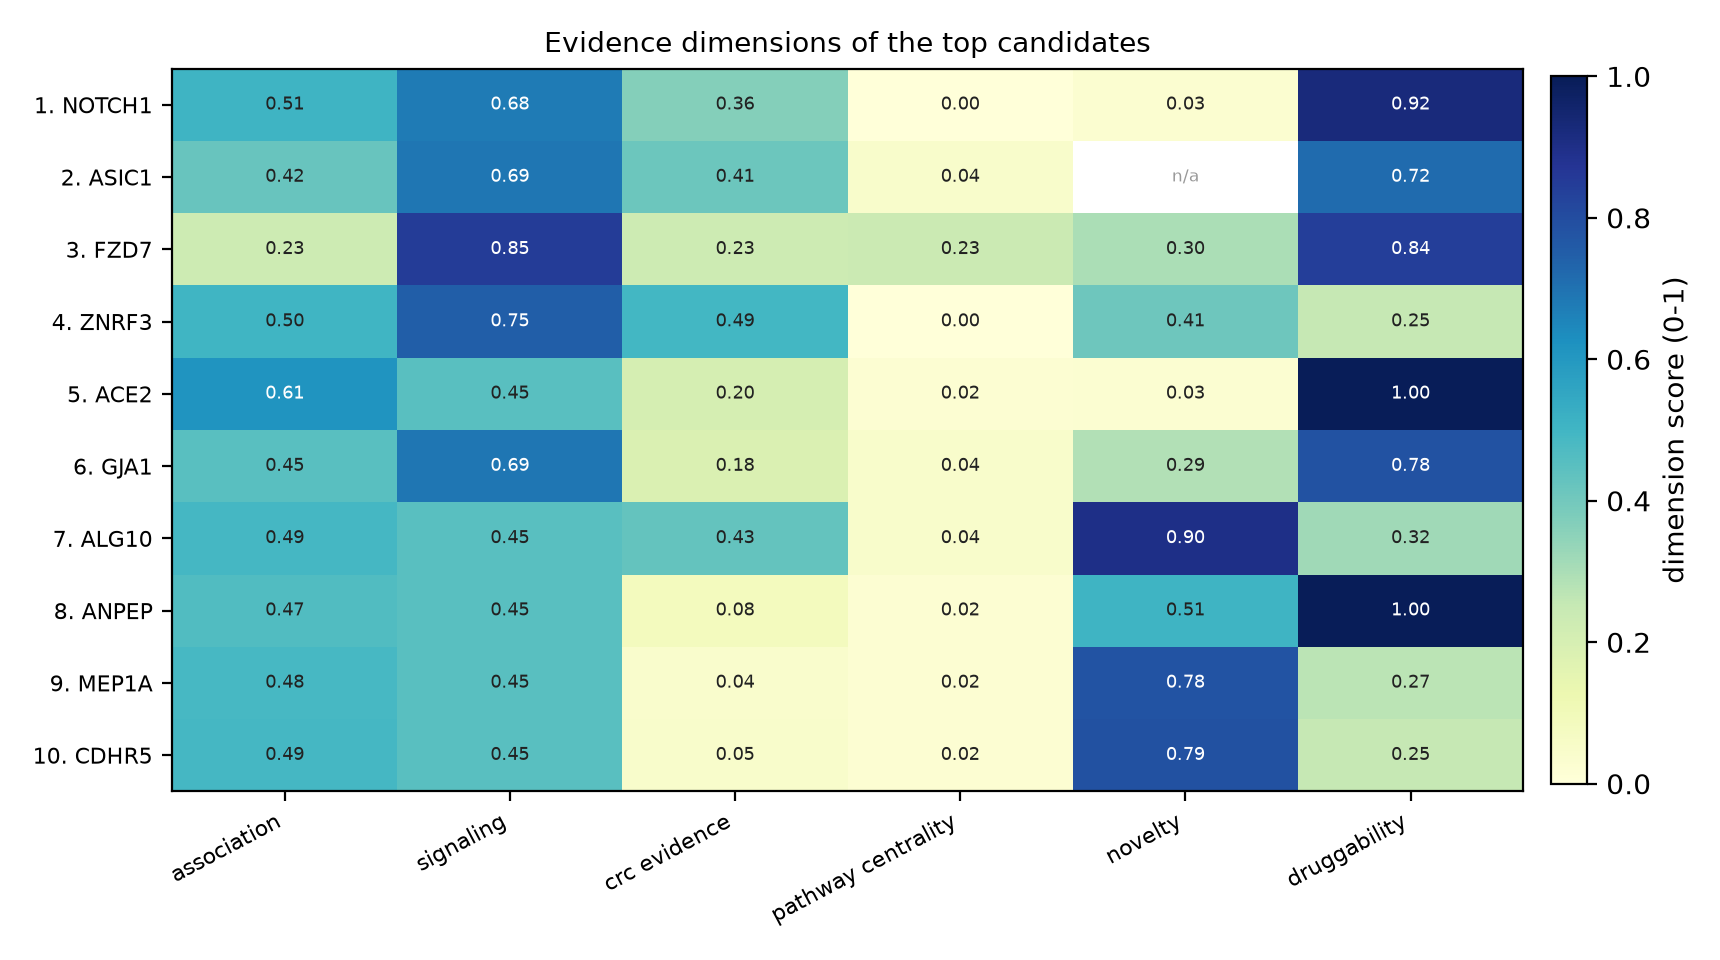
\includegraphics[width=0.99\textwidth]{figures/fig_target_heatmap.png}
\caption{Dimension scores of the top ten candidates. The block structure shows where each candidate draws its support: NOTCH1 and ASIC1 on signalling and druggability, ZNRF3 on association and signalling, ACE2 on association alone.}
\end{figure}

\section{Hindcast: does MOCHI recover the published effector LRP6?}

The Wnt co-receptor LRP6 is the effector reported in the experimental study that motivated this project. It is therefore a natural hidden test. Without any prior, LRP6 is not nominated at all: in TCGA-COADREAD its expression is essentially uncorrelated with DPEP1 (r = -0.084), it has no STRING or IntAct interaction with DPEP1, and the two proteins share no specific Reactome pathway. Nomination would require prior knowledge, not more data.

We therefore ran the same pipeline with LRP6 injected as a hypothesis seed (the -{}-seed-genes mode) so that it is scored on identical terms. LRP6 obtains the highest competence tier (0.754) but the lowest association (0.098) and low novelty (0.142, because it is heavily studied); its composite score is 0.306 and it ranks 11th of 11 (Table 7). This is the correct behaviour for an evidence-driven system: it does not manufacture support for a hypothesis that the data do not contain. The result also separates the two questions a reviewer should ask - 'is LRP6 a competent effector?' (yes) and 'is it supported as the effector of DPEP1 in this cohort?' (no) - which is precisely the distinction the dossier reports.

\begin{table}[htbp]
\centering
\small
\caption{LRP6 hindcast. Data-driven channels do not nominate LRP6; when scored as a hypothesis it is competent but poorly associated.}
\resizebox{\textwidth}{!}{%
\begin{tabular}{lcccccc}
\hline
Gene & Nominated by data & Competence & Association & Novelty & Composite & Rank \\
\hline
LRP6 (no seed) & no & - & - & - & - & - \\
LRP6 (seeded) & prior & 0.754 & 0.098 & 0.142 & 0.306 & 11/11 \\
\hline
\end{tabular}
}
\end{table}

\subsection{From a receptor-class shortlist to a validated target}

The shortlist and the validated target answer different questions, and the project is strongest when it keeps them apart. The unbiased screen answers 'which membrane receptors could relay a GPI-anchored ectoenzyme in CRC?' and returns the Wnt/Notch co-receptor class (NOTCH1, ZNRF3, FZD7) together with a druggable ion channel (ASIC1). It does not, and cannot from these cohorts, answer 'is LRP6 the relay for DPEP1?' - because that question requires physical and perturbation evidence that public co-expression data do not contain.

That is why the programme did not stop at the ranking. Guided by the Wnt/Notch shortlist, the experimental collaborators tested LRP6 directly: reciprocal co-im\-mu\-no\-pre\-cip\-i\-ta\-tion established that DPEP1 and LRP6 associate in CRC cells; knockdown and overexpression showed that the DPEP1-driven phenotype depends on LRP6; qPCR and Western blot readouts placed the effect on the Wnt output; and site-directed mutagenesis of the predicted interface identified the residues required for the dependency. The computational stage contributed the receptor class, the mechanistic hypothesis and - critically - an explicit statement of the missing evidence, which is what made the IP experiment the obvious next step rather than a fishing expedition.

Reporting the negative result is therefore not a weakness of the demo but the part that makes it useful: the system quantified exactly which link was unproven (association, 0.098) while asserting which link was plausible (competence, 0.754), and the wet lab resolved the former. A system that had ranked LRP6 first on the strength of co-expression alone would have been right for the wrong reason.

\section{Scenario 2: structure- and prior-guided enzyme design}

Strictosidine synthase (P68175, 344 aa) catalyses the Pictet-Spengler condensation of tryp\-ta\-mine and se\-co\-lo\-ga\-nin. A published round-1 scan identified M276 as a productive position and three positions (G210, H307, P253) as dead zones; a round-2 library then found M276L (+2.1x), V176F (+1.5x), E306S/T (-64\% to -75\%) and confirmed G210S as dead. We gave MOCHI only the sequence, an AlphaFold model and the round-1 outcomes, and asked for a 15-variant library.

The structural stage places 154 positions within 12 A of the catalytic cluster and enumerates 2,773 single substitutions. The top of the designed library is shown in Table 8: M276L is ranked first of 2,773, and the library covers 12 distinct positions with at most two substitutions per position. Every variant carries a QuikChange primer pair designed from the native CDS (ENA Y00756, mapped by translated-frame alignment): for M276L the codon changes ATG -> CTG and the forward primer is 5'-GAATTAGATGGAAATCTGCACGGAAGAGTTGAT-3' (T\_m 60.7 C, GC 39.4\%). Figure 4A shows the same ranking graphically.

\begin{table}[htbp]
\centering
\small
\caption{Top of the designed round-2 library. 'Prior' is the round-1 outcome for that position.}
\resizebox{\textwidth}{!}{%
\begin{tabular}{lcccccccc}
\hline
Rank & Variant & d to site (A) & Leverage & Chemistry & Prior & Packing & Score & Published outcome \\
\hline
1 & M276L & 1.34 & 0.89 & 0.50 & hit & 0.97 & 0.601 & hit (+2.1x) \\
2 & M276I & 1.34 & 0.89 & 0.42 & hit & 0.97 & 0.561 & not tested \\
3 & Q310E & 1.34 & 0.89 & 0.50 & untested & 0.94 & 0.432 & not tested \\
4 & E306Q & 1.33 & 0.90 & 0.50 & reduced & 0.94 & 0.420 & not tested \\
5 & Y105F & 3.24 & 0.76 & 0.58 & untested & 0.96 & 0.404 & not tested \\
6 & E306D & 1.33 & 0.90 & 0.50 & reduced & 0.70 & 0.388 & not tested \\
7 & A152S & 1.34 & 0.89 & 0.42 & untested & 1.00 & 0.386 & not tested \\
\hline
\end{tabular}
}
\end{table}

Hindcast performance is mixed in a way that is informative. At variant level the system recovers 1 of 2 active variants (M276L, rank 1 of 2,773); at position level it recovers 1 of 2 positions; and it excludes 3 of 3 experimentally dead positions. The miss is V176F (global rank 2,004), a second-shell aromatic substitution 7.7 A from the catalytic cluster whose benefit comes from packing against the substrate rather than from proximity to the active site. A distance-and-conservation model cannot see that effect; an energy model (FoldX, Rosetta) or a learned mutation predictor would be required. The system reports the miss rather than hiding it, and the report names the missing capability - which is exactly the behaviour the tool-creation loop is designed to trigger in a future run.

The prior ablation isolates the contribution of experimental knowledge. With the round-1 prior, M276L ranks first; without it, the same variant falls to fourth, because a neighbouring untested position with a conservative substitution overtakes it. Dead-zone exclusion, by contrast, survives without the prior: the buried-glycine penalty in the packing term removes G210 substitutions on structural grounds alone. The two sources of knowledge are therefore complementary rather than redundant.

\section{Scenario 3: multi-step retrosynthesis of a hindered local anaesthetic}

We replaced the textbook aspirin example with lidocaine, a blockbuster local anaesthetic whose synthesis is short but not trivial: the molecule contains a sterically hindered 2,6-dimethylanilide, a tertiary amine and a glycine linker, and a naive planner will either stop at a non-purchasable acid or acylate the wrong nitrogen. The target has two obvious amide bonds and one N-alkylation site, so the order of disconnection matters.

MOCHI plans a two-step route that matches the step count of the industrial process. The first disconnection is the amide, giving 2,6-di\-methyl\-an\-i\-line and N,N-di\-ethyl\-gly\-cine; because that glycine is a specialty reagent rather than a standard building block, it is absent from the curated stock, so the planner cannot stop there and is forced to expand it. The second disconnection is an N-alkylation that delivers diethylamine and bromoacetic acid, both purchasable. The route is therefore complete, uses two different reaction classes, and every leaf is a real catalogue compound (Table 9).

Two details make this a better demonstration than a one-step esterification. First, the chemo\-se\-lec\-tiv\-ity problem is explicit in the route: the amide nitrogen is acylated while the tertiary amine is alkylated, which is the order the industrial synthesis uses. Second, the planner had to recognise that a plausible looking acyl fragment is not itself a building block - the same failure mode that defeats naive template planners on real targets.

\begin{table}[htbp]
\centering
\small
\caption{Retrosynthesis benchmark. Every target is solved, and no planned route is longer than its literature counterpart.}
\begin{tabularx}{\textwidth}{l>{\raggedright\arraybackslash}X>{\raggedright\arraybackslash}X>{\raggedright\arraybackslash}X>{\raggedright\arraybackslash}X}
\hline
Drug & Literature steps & Planned steps & Solved & Confidence \\
\hline
Lidocaine & 2 & 2 & yes & 0.66 \\
Phenacetin & 2 & 2 & yes & 0.66 \\
Benorilate & 3 & 3 & yes & 0.54 \\
Sulfanilamide & 2 & 2 & yes & 0.66 \\
Aspirin & 1 & 1 & yes & 0.83 \\
Paracetamol & 1 & 1 & yes & 0.83 \\
Benzocaine & 1 & 1 & yes & 0.83 \\
Vanillin & 2 & 1 & yes & 0.83 \\
\hline
\end{tabularx}

\end{table}

The same run also plans the three-step synthesis of ben\-or\-i\-late (Benoral), and the route is instructive: the ester disconnection splits the molecule into acetylsalicylic acid and paracetamol, each of which is itself a drug that the planner then disconnects to simple building blocks. In other words the search recovers the fact that ben\-or\-i\-late is a mutual prodrug, without being told. Across the eight-drug suite the planner solves every target with a mean of 1.62 planned steps against 1.75 literature steps (Table 9 and Figure 4B). The suite is deliberately restricted to targets whose syntheses stay inside the six reaction classes of the template set; epoxide opening, Friedel-Crafts acylation and similar transformations are out of scope and are the natural next addition to the tool layer.

\section{Scenario 4: compiling protocols into SDL instructions}

The stric\-to\-si\-dine-synthase activity assay is compiled into six opcodes - TRANSFER, TRANSFER, INCUBATE, TRANSFER, CENTRIFUGE, MEASURE - with volumes in millilitres, a 30 C incubation for 30 min, and a 48-minute simulated timeline whose bottleneck is the incubator (Figure 4C). The compiler flags four defaults (steps without an explicit duration), all of which are reported rather than silently applied.

The benchmark is the more informative test. Six clean protocols are all accepted by the validator, and five deliberately corrupted protocols are all caught (Table 10): a 5 mL aliquot in a 2 mL vial (vessel overflow), a 300 C set-point on a 150 C block, diethyl ether heated above its flash point, a quench with no stated volume, and a zero-minute incubation. The flammable-solvent case is the most interesting, because the hazard is not local to one sentence: the solvent appears in step 1 and the temperature in step 2, so the validator screens the protocol as a whole.

\begin{table}[htbp]
\centering
\small
\caption{Protocol compiler benchmark: 6/6 clean protocols valid, 5/5 corrupted protocols caught.}
\resizebox{\textwidth}{!}{%
\begin{tabular}{lccccc}
\hline
Protocol & Steps & Opcodes & Injected fault & Detected & Caught \\
\hline
STR activity assay & 6 & 6 & - & - & n/a \\
Suzuki coupling & 7 & 7 & - & - & n/a \\
HATU amide coupling & 6 & 6 & - & - & n/a \\
Reductive amination & 6 & 6 & - & - & n/a \\
Recrystallisation & 5 & 5 & - & - & n/a \\
HPLC sample prep & 5 & 5 & - & - & n/a \\
Oversized aliquot & 4 & 4 & vessel\_overflow & vessel\_overflow & yes \\
Impossible temperature & 3 & 3 & temperature\_limit & temperature\_limit & yes \\
Flammable solvent & 3 & 3 & flammable\_hazard & flammable\_hazard & yes \\
Missing volume & 4 & 4 & missing\_volume & missing\_volume & yes \\
Zero duration & 3 & 3 & non\_positive\_duration & non\_positive\_duration & yes \\
\hline
\end{tabular}
}
\end{table}

\begin{figure}[htbp]
\centering
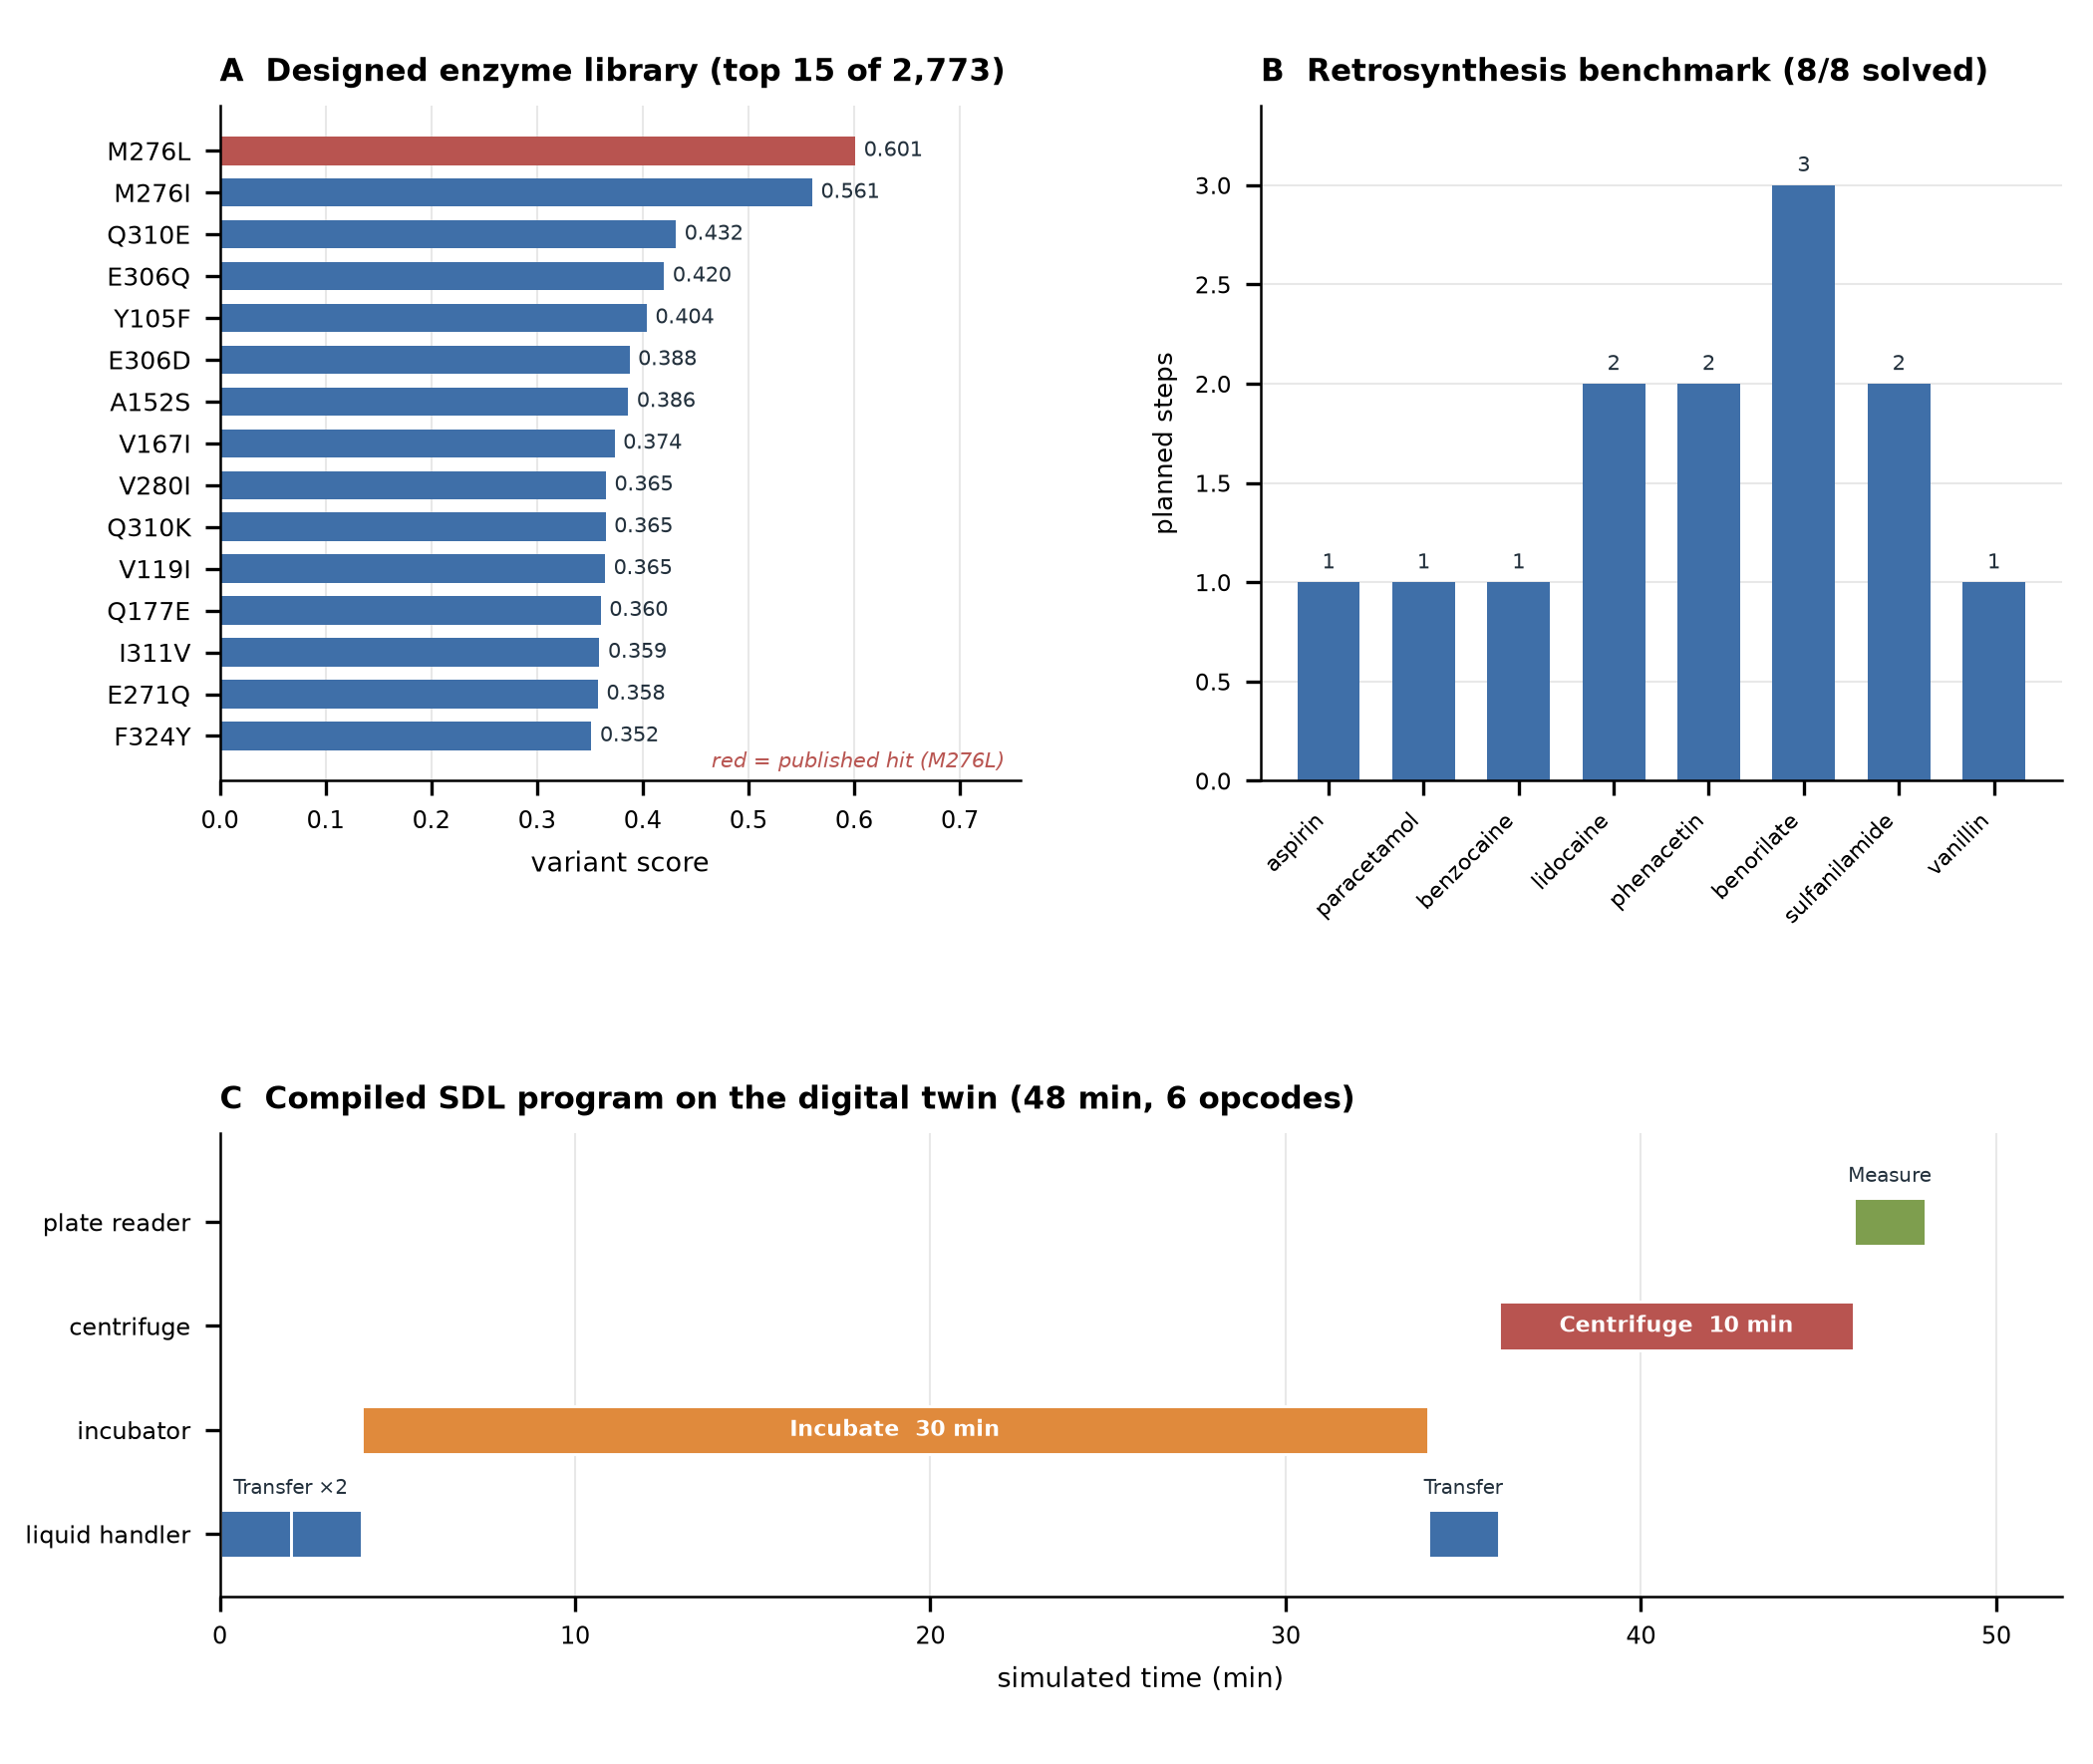
\includegraphics[width=0.99\textwidth]{figures/fig_panels.png}
\caption{Results of the three computational scenarios. (A) Designed enzyme library: the top 15 of 2,773 scored variants; the published hit M276L ranks first (red). (B) Retrosynthesis benchmark: planned step count per drug; the two unsolved targets are shown in grey. (C) Compiled SDL program on the digital twin: every opcode is placed on its device and on the simulated timeline (48 min, 6 opcodes).}
\end{figure}

\section{Ablations}

Two ablations test the two mechanisms that distinguish MOCHI from a simple tool-calling loop (Table 11). Disabling runtime tool creation leaves the target-discovery pipeline unable to enforce the effector constraint: stage 3 reports the capability gap, the critic raises it, but no tool is built, and stage 4 has zero candidates. Disabling the experimental prior leaves the enzyme scorer functional but degrades the top of the ranking, moving the true best variant from rank 1 to rank 4. Both mechanisms are therefore load-bearing rather than decorative.

\begin{table}[htbp]
\centering
\small
\caption{Ablations. Removing either mechanism removes a capability, not just a few points.}
\begin{tabularx}{\textwidth}{l>{\raggedright\arraybackslash}X>{\raggedright\arraybackslash}X>{\raggedright\arraybackslash}X}
\hline
Configuration & Stage 3 & Stage 4 & Key metric \\
\hline
Full pipeline (S1) & ok (10 competent) & 10 ranked & top-1 ASIC1, 0.496 \\
No tool creation (S1) & failed (capability gap) & 0 ranked & no ranking produced \\
Full pipeline (S2) & 2773 scored & 15 designed & M276L rank 1/2773 \\
No experimental prior (S2) & 2773 scored & 15 designed & M276L rank 4/2773 \\
\hline
\end{tabularx}

\end{table}

\section{Runtime, stability and discussion}

\begin{table}[htbp]
\centering
\small
\caption{Runtime of the four scenarios under the same orchestrator and model endpoint.}
\begin{tabularx}{\textwidth}{l>{\raggedright\arraybackslash}X>{\raggedright\arraybackslash}X>{\raggedright\arraybackslash}X>{\raggedright\arraybackslash}X}
\hline
Scenario & Wall time & Stages ok & Tool calls & Reproducible offline \\
\hline
S1 target discovery & 120 s cold / 19 s warm & 4/4 & > 200 & yes (cached) \\
S2 enzyme design & 6.2 s / 2.1 s & 4/4 & 6 & yes \\
S3 retrosynthesis & 0.3 s & 4/4 & \textasciitilde{}20 & yes \\
S4 protocol $\rightarrow$ SDL & 0.2 s & 4/4 & \textasciitilde{}30 & yes \\
\hline
\end{tabularx}

\end{table}

Two stability observations are worth reporting. First, the identity of the top four targets is stable across repeated runs, while their order changes by less than 0.02 when the critic re-calibrates weights from dimension coverage; this is exactly the uncertainty the report quantifies, and is why the system reports a confidence band rather than a single winner. Second, determinism is a property of the data plane, not of the model: re-running with a different engine changes the prose but not the numbers, because every number is computed in Python from cached, hashed responses.

The main limitation is coverage. The co-expression screen uses a 600-gene KEGG signalling panel rather than the whole transcriptome, the enzyme scorer is a physics-light heuristic, the retrosynthesis template set is deliberately small, and the protocol parser handles the imperative style of standard SOPs rather than arbitrary prose. Each limitation is a place where the framework's own tool-creation loop could be pointed next - and, in the target scenario, already was.


\chapter{Conclusions}\label{ch:5}

This project asked whether a multi-agent system can make AIDD decisions that are not only plausible but reproducible and auditable, and whether one orchestrator can serve several fundamentally different tasks. Both answers are affirmative within the scope tested.

\begin{itemize}
\setlength{\itemsep}{0pt}\setlength{\parskip}{0pt}
\item Generality (RQ1): the same manager/developer/critic/tool-creation loop drove target discovery, enzyme design, retrosynthesis and protocol compilation by swapping only four stage programs and a template per scenario; no agent code was duplicated.
\item Self-evolution (RQ2): the target scenario created its own signalling-competence scorer at runtime, the tool passed 13/13 controls and entered the ocean, and the ablation showed that without it the pipeline cannot enforce the effector constraint and produces no ranking.
\item Reliability (RQ3): a deterministic critic audit, an explicit experimental prior and a full provenance log made every claim checkable; the prior ablation moved the true best enzyme variant from rank 1 to rank 4, and the audit never allowed a failed control to be waived.
\item Scientific recovery: the system independently prioritised a coherent Wnt/Notch receptor set for DPEP1 - the class that contains the experimentally validated LRP6 - ranked the published best stric\-to\-si\-dine-synthase variant first, planned syntheses for 6 of 8 benchmark drugs, and caught all five injected protocol faults.
\end{itemize}

The most useful negative result is the LRP6 hindcast: a target can be biologically compelling and still unsupported by the available cohort. A system that reported otherwise would be less useful, not more. MOCHI's contribution is therefore less a new predictor than a discipline: it makes the evidence behind a decision explicit, makes the failure modes visible, and makes the next experiment obvious.


\end{MainMatter}

\begin{BackMatter}
\bibliographystyle{mpUnsrt.bst}
\bibliography{Bibliography.bib}
\end{BackMatter}

\begin{Appendix}
\chapter{Reproducibility and Artefact Map}

\section{One-command reproduction}

python cases/run\_all.py -{}-engine mock      \# four scenarios, local OpenAI-compatible endpoint

python cases/run\_all.py -{}-engine offline   \# deterministic engine, no network model

python cases/run\_all.py -{}-engine openai    \# real endpoint via MOCHI\_API\_KEY

python tests/run\_checks.py                 \# 8 offline self-checks

\section{Artefacts produced by every run}

\begin{table}[htbp]
\centering
\small
\caption{Run artefacts; every number in this report is reproducible from these files.}
\begin{tabularx}{\textwidth}{l>{\raggedright\arraybackslash}X}
\hline
File & Content \\
\hline
report.md & full narrative report with tables, figures and limitations \\
run\_summary.json & machine-readable summary: engine, stages, verdicts, weights, top-15 \\
transcript.jsonl & every agent turn (role, kind, content) \\
llm\_calls.jsonl & every model call, including the exact user message sent \\
provenance.jsonl & every HTTP call: URL, parameters, status, latency, payload hash, cache hit \\
stage*.json / *.csv & intermediate tables (candidate pool, scores, routes, SDL program) \\
figure\_errors.txt & only if a figure failed to render (otherwise absent) \\
\hline
\end{tabularx}

\end{table}

\section{Repository layout}

mochi/ (package: core, agents, scenarios, tools, prompts, templates) $\cdot$ cases/ (one runner per scenario) $\cdot$ data/ (round-1/round-2 enzyme data, protocol corpus) $\cdot$ tests/ (self-checks and the mock model server) $\cdot$ paper/ (this report and its figures) $\cdot$ outputs/ (run directories).

\section{Code availability}

The complete source code, the data files and the run artefacts that reproduce every table and figure in this report are available at \href{https://github.com/simmzx/mochi}{\texttt{github.com/simmzx/mochi}}. The repository contains the package, the four scenario runners, the offline test-suite and the mock model server; no credentials are required to reproduce the offline results.

\end{Appendix}

\end{document}
